\documentclass[11pt,a4paper]{ctexart}
\usepackage[teacher]{../ipara}
% =====================================================
% 模板测试/样例题目组装 (questions.tex)
% =====================================================

% 引入公共核心题库中的题目
% =====================================================
% 题型：立体几何多结论选择题 (q1_solid_mc.tex)
% =====================================================
% =====================================================
% 难度：★★ (中档)
% =====================================================
\newcommand{\qOneStem}{如图，\(AB\) 是 \(\odot O\) 的直径，\(PA \perp \text{平面 } \odot O\)，\(C\) 是圆周上不同于 \(A,B\) 的任意一点，则}

\newcommand{\qOneOptions}{%
  \mcoptions[1]{
    若 $D$ 为 $BC$ 的中点，则 $OD \parallel$ 平面 $PAC$
  }{
    平面 $PAC \perp$ 平面 $PBC$
  }{
    点 $A$ 到平面 $PBC$ 的距离小于 $\frac{1}{2} PC$
  }{
    $PB$ 为三棱锥 $P-ABC$ 外接球的直径
  }%
}

\newcommand{\qOneFigure}[1][1.2]{%
  \begin{tikzpicture}[scale=#1, >=stealth]
    \coordinate (O) at (1.2, 0);
    \coordinate (A) at (0, 0);
    \coordinate (B) at (2.4, 0);
    \coordinate (P) at (0, 1.8);
    \coordinate (C) at (0.7, 0.25);
    \coordinate (O1) at (1.2, 1.8);
    \coordinate (Ctop) at (0.7, 2.05);
    
    \draw[thick] (2.4,0) arc (0:-180:1.2 and 0.35);
    \draw[dashed] (2.4,0) arc (0:180:1.2 and 0.35);
    
    \draw[dashed] (1.2,1.8) ellipse (1.2 and 0.35);
    \draw[dashed] (2.4,0) -- (2.4,1.8);
    \draw[dashed] (O) -- (O1);
    \draw[dashed] (C) -- (Ctop);
    
    \draw[thick] (P) -- (A);
    \draw[thick] (P) -- (B);
    \draw[thick, dashed] (P) -- (C);
    \draw[thick, dashed] (A) -- (C);
    \draw[thick, dashed] (C) -- (B);
    \draw[thick] (A) -- (B);
    
    \node[left] at (A) {\small $A$};
    \node[right] at (B) {\small $B$};
    \node[above left] at (P) {\small $P$};
    \node[below] at (O) {\small $O$};
    \node[below right] at (C) {\small $C$};
  \end{tikzpicture}%
}
        % 第一题：立体几何多结论选择题
% =====================================================
% 题型：解三角形求角选择题 (q2_triangle_angle.tex)
% =====================================================
% =====================================================
% 难度：★ (基础)
% =====================================================
\newcommand{\qTwoStem}{在 \(\triangle ABC\) 中，角 \(A, B, C\) 的对边分别为 \(a, b, c\)。若 \(a \cos B + b \cos A = 2c \cos C\)，则角 \(C =\) \hfill （\quad）}

\newcommand{\qTwoOptions}{%
  \mcoptions[4]{\(\dfrac{\pi}{6}\)}{\(\dfrac{\pi}{3}\)}{\(\dfrac{\pi}{2}\)}{\(\dfrac{2\pi}{3}\)}%
}
  % 第二题：解三角形求角选择题
% =====================================================
% 题型：平面向量夹角选择题 (q3_vector_angle.tex)
% =====================================================
% =====================================================
% 难度：★ (基础)
% =====================================================
\newcommand{\qThreeStem}{已知非零向量 \(\vec{a}, \vec{b}\) 满足 \(|\vec{a}| = 1\), \(|\vec{b}| = 2\)，且 \(\vec{a} \cdot (\vec{a} + \vec{b}) = 2\)，则向量 \(\vec{a}\) 与 \(\vec{b}\) 的夹角为 \hfill （\quad）}

\newcommand{\qThreeOptions}{%
  \mcoptions[4]{\(\dfrac{\pi}{6}\)}{\(\dfrac{\pi}{4}\)}{\(\dfrac{\pi}{3}\)}{\(\dfrac{2\pi}{3}\)}%
}
    % 第三题：平面向量夹角选择题
% =====================================================
% 题型：立体几何解答题 (q4_pyramid_proof.tex)
% =====================================================
% =====================================================
% 难度：★★★ (难题)
% =====================================================
\newcommand{\qFourStem}{%
  如图，在四棱锥 $P-ABCD$ 中，$AB\parallel CD$，且 $\angle BAP=\angle CDP=90^\circ$。
  \begin{enumerate}[label=(\arabic*) , leftmargin=2em, itemsep=0.1em]
    \item 证明：平面 $PAB\perp$ 平面 $PAD$；
    \item 若 $PA=PD=AB=DC$，$\angle APD=90^\circ$，且四棱锥 $P-ABCD$ 的体积为 $\dfrac{8}{3}$，求 $PB$ 与平面 $ABCD$ 所成角的大小。
  \end{enumerate}%
}

\newcommand{\qFourFigure}[1][1.1]{%
  \begin{tikzpicture}[scale=#1, >=stealth]
    \coordinate (A) at (0, 0);
    \coordinate (B) at (0.8, -0.6);
    \coordinate (C) at (2.8, -0.6);
    \coordinate (D) at (2.0, 0);
    \coordinate (P) at (1.0, 1.5);
    
    \draw[thick] (P) -- (A);
    \draw[thick] (P) -- (B);
    \draw[thick] (P) -- (C);
    \draw[thick, dashed] (P) -- (D);
    \draw[thick] (A) -- (B);
    \draw[thick] (B) -- (C);
    \draw[thick, dashed] (C) -- (D);
    \draw[thick, dashed] (A) -- (D);
    
    \ifteacher
      \coordinate (H) at (1.0, 0);
      % 教师教案专属：辅助投影高线 PH 与投影线 BH
      \draw[semithick, dashed, gray] (P) -- (H);
      \draw[semithick, dashed, gray] (B) -- (H);
      \node[above right] at (H) {\small $H$};
    \fi
    
    \node[left] at (A) {\small $A$};
    \node[below left] at (B) {\small $B$};
    \node[below right] at (C) {\small $C$};
    \node[above right] at (D) {\small $D$};
    \node[above] at (P) {\small $P$};
  \end{tikzpicture}%
}
   % 第四题：立体几何解答题


% =====================================================
% 页眉页脚设置（教案端）
% =====================================================
\pagestyle{fancy}
\fancyhf{}
\lhead{\small 专题复习教案（教师备课用）}
\rhead{\small 专题：立体几何、平面向量与解三角形}
\cfoot{\small 第 \thepage\ 页\quad 共 \pageref{LastPage} 页}
\renewcommand{\headrulewidth}{0.4pt}
\renewcommand{\footrulewidth}{0pt}


\begin{document}

% =====================================================
% 页头设计
% =====================================================
\begin{center}
  {\Large\bfseries 专题复习教案}\\
  \vspace{0.6em}
  {\large 教师备课专用\quad 专题：立体几何、平面向量与解三角形}
\end{center}

\section{教学目标与重难点}
\textbf{【教学目标】}
\begin{enumerate}[label=\arabic*. , leftmargin=2em, itemsep=0.1em, topsep=0.2em]
  \item 熟练掌握线面平行、线面垂直、面面垂直的判定定理与性质定理。
  \item 熟练应用正弦定理、余弦定理进行三角形内“边角互化”及代数式化简。
  \item 熟练运用平面向量数量积展开式及夹角公式求解模长与角度。
  \item 培养学生空间想象力、代数推推导精度以及规范书写解答题逻辑链的习惯。
\end{enumerate}

\vspace{0.8em}
\textbf{【教学重难点】}
\begin{description}[leftmargin=2em, itemsep=0.1em, topsep=0.2em]
  \item[重点] 解答题中线面垂直证明步骤的逻辑严密性（“相交”与“线在面内”条件的书写）；线面角的空间构造与计算。
  \item[难点] 圆柱内接三棱锥外接球的几何感知；向量数量积与三角恒等变换在复杂表达式中的综合处理。
\end{description}

\newpage

\section{备课公式与方法库}

\subsection{本节必讲公式}
作为全体学生必须掌握的基础主线，要求在课堂导入与二次默写中进行严密监控：

\begin{enumerate}[label=\arabic*. , leftmargin=2em, itemsep=1.2em, topsep=0.2em]
  \item \textbf{线面垂直判定定理}：一条直线垂直于平面内的两条相交直线，则这条直线垂直于该平面。
  数理表达：
  \[
  \left.
  \begin{aligned}
    l &\perp a \\
    l &\perp b \\
    a &\cap b = P \\
    a, b &\subset \alpha
  \end{aligned}
  \right\} \implies l \perp \alpha
  \]
  \begin{center}
    \begin{tikzpicture}[scale=1.1, >=stealth]
      \draw[thick] (0,0) -- (3,0) -- (4,1.2) -- (1,1.2) -- cycle;
      \node at (3.6,0.3) {$\alpha$};
      \coordinate (P) at (2.2, 0.6);
      \coordinate (Ltop) at (2.2, 2.0);
      \coordinate (Pa) at (3.2, 0.9);
      \coordinate (Pb) at (2.9, 0.2);
      \draw[thick, dashed, gray] (1.2, 0.3) -- (Pa) node[right, black] {$a$};
      \draw[thick, dashed, gray] (1.5, 1.0) -- (Pb) node[right, black] {$b$};
      \fill (P) circle (1.5pt) node[below] {\small $P$};
      \draw[thick, black] (P) -- (Ltop) node[above] {$l$};
      \draw[thick, dashed, black] (P) -- (2.2, -0.4);
      
      % Right angle markers (3D style)
      \coordinate (P1) at ($(P)!0.15!(Ltop)$);
      \coordinate (P2) at ($(P)!0.15!(Pa)$);
      \coordinate (P3) at ($(P1)+(P2)-(P)$);
      \draw[very thin] (P1) -- (P3) -- (P2);
      
      \coordinate (P4) at ($(P)!0.15!(Pb)$);
      \coordinate (P5) at ($(P1)+(P4)-(P)$);
      \draw[very thin] (P1) -- (P5) -- (P4);
    \end{tikzpicture}
    \par\vspace{0.2em}
    {\small\textbf{图 2.1 线面垂直判定示意图}}
  \end{center}
  
  \item \textbf{面面垂直判定定理}：一个平面内有一条直线垂直于另一个平面，则这两个平面相互垂直。
  数理表达：
  \[
  \left.
  \begin{aligned}
    l &\subset \beta \\
    l &\perp \alpha
  \end{aligned}
  \right\} \implies \beta \perp \alpha
  \]
  \begin{center}
    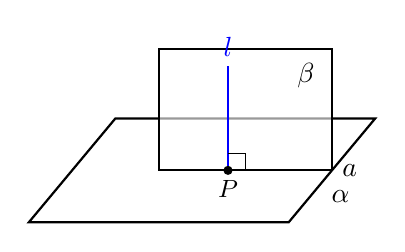
\begin{tikzpicture}[scale=1.1, >=stealth]
      \draw[thick] (0,0) -- (3,0) -- (4,1.2) -- (1,1.2) -- cycle;
      \node at (3.6,0.3) {$\alpha$};
      \draw[thick, fill=white, fill opacity=0.6] (1.5,0.6) -- (1.5,2.0) -- (3.5,2.0) -- (3.5,0.6) -- cycle;
      \node at (3.2,1.7) {$\beta$};
      \draw[thick, dashed] (1.5,0.6) -- (3.5,0.6) node[right, black] {$a$};
      \draw[thick, blue] (2.3, 0.6) -- (2.3, 1.8) node[above] {$l$};
      \fill (2.3, 0.6) circle (1.5pt) node[below] {\small $P$};
      \draw (2.3, 0.8) -- (2.5, 0.8) -- (2.5, 0.6);
    \end{tikzpicture}
    \par\vspace{0.2em}
    {\small\textbf{图 2.2 面面垂直判定示意图}}
  \end{center}

  \item \textbf{棱锥体积公式}：
  \[
  V = \frac{1}{3} S_{\text{底}} h_{\text{高}}
  \]
  其中 $S_{\text{底}}$ 为底面多边形的面积，$h_{\text{高}}$ 为顶点到底面的距离（高）。
  课堂强调：
  \begin{itemize}[label=\(\circ\), leftmargin=1.5em, itemsep=0.1em]
    \item 前置系数 \(\frac{1}{3}\) 是学生大题中最容易漏写的关键项，必须强力提醒。
    \item 底面积 $S_{\text{底}}$ 计算往往与解三角形（如 \(S = \frac{1}{2}ab\sin C\)）或特殊四边形相结合。
  \end{itemize}

  \item \textbf{线面角定义与“作—证—算”}：
  一条斜线与平面所成的角，是该斜线与它在平面内的射影所成的角。
  数理表达：
  若 $PH \perp \alpha$，$H$ 为垂足，$A$ 为斜线与平面的交点，则 $AH$ 为斜线 $PA$ 在平面 $\alpha$ 内的射影，$\theta = \angle PAH$ 即为斜线 $PA$ 与平面 $\alpha$ 所成角。
  \begin{center}
    \begin{tikzpicture}[scale=1.1, >=stealth]
      \draw[thick] (0,0) -- (3,0) -- (4,1.2) -- (1,1.2) -- cycle;
      \node at (3.6,0.3) {$\alpha$};
      \coordinate (A) at (1.2, 0.4);
      \coordinate (H) at (2.8, 0.6);
      \coordinate (P) at (2.8, 1.8);
      \draw[thick] (A) -- (P) node[above] {$P$};
      \draw[thick, dashed] (A) -- (H) node[below] {$H$};
      \draw[thick] (P) -- (H);
      \node[left] at (A) {$A$};
      \draw (1.5, 0.44) arc (8:35:0.5);
      \node at (1.8, 0.55) {$\theta$};
      \fill (A) circle (1.2pt);
      \fill (H) circle (1.2pt);
      \fill (P) circle (1.2pt);
      
      % Right angle at H (3D style)
      \coordinate (H1) at ($(H)!0.15!(P)$);
      \coordinate (H2) at ($(H)!0.15!(A)$);
      \coordinate (H3) at ($(H1)+(H2)-(H)$);
      \draw[very thin] (H1) -- (H3) -- (H2);
    \end{tikzpicture}
    \par\vspace{0.2em}
    {\small\textbf{图 2.3 线面角示意图}}
  \end{center}
  教学规范步骤（“作—证—算”）：
  \begin{description}[leftmargin=1.5em, itemsep=0.1em]
    \item[作] 作出顶点的投影，指明射影，标出夹角。
    \item[证] 严密证明所找的线为高（线面垂直），进而证明该角为所求。
    \item[算] 放入对应的直角三角形中求出三角函数值，最终解出夹角。
  \end{description}

  \item \textbf{向量夹角公式}：
  对于非零向量 \(\vec{u}, \vec{v}\)，其夹角 \(\theta \in [0, \pi]\) 满足：
  \[
  \cos\theta = \frac{\vec{u} \cdot \vec{v}}{|\vec{u}||\vec{v}|}
  \]
  若使用坐标表示，设 \(\vec{u} = (x_1, y_1), \vec{v} = (x_2, y_2)\)，则：
  \[
  \cos\theta = \frac{x_1x_2 + y_1y_2}{\sqrt{x_1^2+y_1^2}\sqrt{x_2^2+y_2^2}}
  \]
  重点强调：注意区分数量积正负与夹角大小的关系：
  \begin{itemize}[label=\(\circ\), leftmargin=1.5em, itemsep=0.1em]
    \item \(\vec{u}\cdot\vec{v} > 0 \iff \theta \in [0, \frac{\pi}{2})\)（夹角为锐角或零角）；
    \item \(\vec{u}\cdot\vec{v} < 0 \iff \theta \in (\frac{\pi}{2}, \pi]\)（夹角为钝角或平角，排除反向共线需要看模长关系）。
  \end{itemize}
\end{enumerate}

\subsection{高分拓展结论}
适合中高分段学生作解题方法的拔高训练，主要用于提升高考或考前模拟中的解题速度：

\begin{enumerate}[label=\arabic*. , leftmargin=2em, itemsep=1.2em, topsep=0.2em]
  \item \textbf{射影定理（第一余弦定理）}：
  在 \(\triangle ABC\) 中，有：
  \[
  c = a\cos B + b\cos A,\quad a = b\cos C + c\cos B,\quad b = c\cos A + a\cos C
  \]
  几何意义：三角形某一边的长度等于另外两边在改边上的射影长度之和。本案第2题中，代数式 \(a\cos B + b\cos A\) 可直接利用此定理代换为 \(c\)，从而极速化简。

  \item \textbf{直角共斜边外接球模型}：
  若空间四点 $P, A, B, C$ 满足 $\angle PAB = \angle PCB = 90^\circ$，则该三棱锥的外接球以公共斜边 $PB$ 为直径，球心 $O$ 为 $PB$ 的中点，外接球半径 $R = \frac{1}{2}PB$。
  \begin{center}
    \begin{tikzpicture}[scale=1.3, >=stealth]
      % Draw sphere circle
      \draw[thick] (0,0) circle (1.8);
      % Equator ellipse (3D effect)
      \draw[dashed, gray] (0,0) ellipse (1.8 and 0.55);
      
      % Coordinates
      \coordinate (O) at (0,0);
      \coordinate (P) at (-1.56, -0.9);
      \coordinate (B) at (1.56, 0.9);
      \coordinate (A) at (-0.3, 1.77);  % On sphere boundary
      \coordinate (C) at (0.8, -0.49);  % On equator ellipse
      
      % Draw diameter PB
      \draw[thick, blue] (P) -- (B) node[midway, above left, black] {$O$};
      % Draw triangles
      \draw[thick] (P) -- (A) node[above left] {$A$};
      \draw[thick] (B) -- (A);
      \draw[thick] (P) -- (C) node[below right] {$C$};
      \draw[thick] (B) -- (C);
      \draw[dashed] (A) -- (C);
      
      % Label P and B
      \node[below left] at (P) {$P$};
      \node[above right] at (B) {$B$};
      \fill (O) circle (1.5pt);
      
      % Right angle at A (3D style)
      \coordinate (A1) at ($(A)!0.15!(P)$);
      \coordinate (A2) at ($(A)!0.15!(B)$);
      \coordinate (A3) at ($(A1)+(A2)-(A)$);
      \draw[very thin] (A1) -- (A3) -- (A2);
      
      % Right angle at C (3D style)
      \coordinate (C1) at ($(C)!0.15!(P)$);
      \coordinate (C2) at ($(C)!0.15!(B)$);
      \coordinate (C3) at ($(C1)+(C2)-(C)$);
      \draw[very thin] (C1) -- (C3) -- (C2);
    \end{tikzpicture}
    \par\vspace{0.2em}
    {\small\textbf{图 2.4 直角共斜边外接球模型示意图}}
  \end{center}

  \item \textbf{直棱柱补形法与半径公式}：
  对于直棱柱、圆柱或其内接多面体，其外接球与原多面体共用同一个外接球，外接球半径满足：
  \[
  R = \sqrt{r^2 + \left(\frac{h}{2}\right)^2}
  \]
  其中 $r$ 为底面多边形外接圆的半径，$h$ 为直棱柱或圆柱的高。若底面为 $\triangle ABC$，则底面外接圆半径可通过正弦定理计算：
  \[
  r = \frac{a}{2\sin A} = \frac{b}{2\sin B} = \frac{c}{2\sin C}
  \]
\end{enumerate}

\subsection{教师备查结论}
教师备课参考，视课堂进度或竞赛性拓展需求灵活使用，不作全体讲解要求：

\begin{enumerate}[label=\arabic*. , leftmargin=2em, itemsep=1.2em, topsep=0.2em]
  \item \textbf{中点形式的极化恒等式}：
  设 $M$ 为线段 $BC$ 的中点，对于平面内任意一点 $A$，恒有：
  \[
  \vec{AB} \cdot \vec{AC} = \vec{AM}^2 - \frac{1}{4}\vec{BC}^2
  \]
  极化恒等式将向量的数量积计算转化为向量模长的平方差。在解决“起点固定、终点在线段上滑动”的数量积极值与最值问题时极为高效。
  \begin{center}
    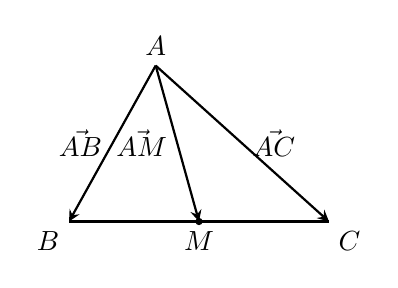
\begin{tikzpicture}[scale=1.1, >=stealth]
      \coordinate (B) at (0,0);
      \coordinate (C) at (3,0);
      \coordinate (M) at (1.5,0);
      \coordinate (A) at (1.0,1.8);
      \draw[thick, ->] (A) -- (B) node[midway, left] {$\vec{AB}$};
      \draw[thick, ->] (A) -- (C) node[midway, right] {$\vec{AC}$};
      \draw[thick, ->] (A) -- (M) node[midway, left] {$\vec{AM}$};
      \draw[thick] (B) -- (C);
      \node[below left] at (B) {$B$};
      \node[below right] at (C) {$C$};
      \node[below] at (M) {$M$};
      \node[above] at (A) {$A$};
      \fill (M) circle (1.2pt);
    \end{tikzpicture}
    \par\vspace{0.2em}
    {\small\textbf{图 2.5 中点形式极化恒等式示意图}}
  \end{center}

  \item \textbf{奔驰定理}：
  若 $O$ 是 $\triangle ABC$ 内任意一点，其面积关系与向量关系满足：
  \[
  S_{\triangle BOC}\vec{OA} + S_{\triangle AOC}\vec{OB} + S_{\triangle AOB}\vec{OC} = \vec{0}
  \]
  该定理将点 $O$ 在三角形内的几何面积关系直接转化为向量线性组合形式。
  
  \item \textbf{阿波罗尼斯圆}：
  若动点 $P$ 到两定点 $A, B$ 的距离之比 $\frac{PA}{PB} = \lambda$ ($\lambda > 0$ 且 $\lambda \neq 1$)，则动点 $P$ 的轨迹为一圆。
  代数方程形式：在平面直角坐标系中，设 $A(d, 0), B(-d, 0)$，则 $P(x,y)$ 满足：
  \[
  \frac{(x-d)^2+y^2}{(x+d)^2+y^2} = \lambda^2
  \]
  化简后可得一标准圆方程，圆心在 $AB$ 所在直线上。
\end{enumerate}

\newpage

% =====================================================
% 核心题型精讲（双栏对比版式）
% =====================================================
\section{核心题型精讲与诊断}

% -----------------------------------------------------
% 第一题详案
% -----------------------------------------------------
\teachquestionheader{立体几何多结论选择题}

\begin{minipage}[t]{0.7\textwidth}
  \vspace{0pt}
  \qOneStem 以下结论正确的是 \blank{1.5cm}
  \qOneOptions
\end{minipage}
\hfill
\begin{minipage}[t]{0.26\textwidth}
  \vspace{0pt}
  \hfill
  \qOneFigure[0.95]
\end{minipage}

\vspace{0.8em}

\begin{paracol}{2}
  \textbf{【考查意图】}\\
  考查空间线面、面面垂直的判定方法与圆周角性质的结合；考查直三棱锥外接球的球心几何定位方法。
  
  \textbf{【课堂主线】}\\
  底面圆直径 $\to AC \perp BC$ $\to$ 结合 $PA \perp$ 底面 $\implies PA \perp BC$ $\to$ 线面垂直判定 $BC \perp$ 平面 $PAC$ $\to$ 面面垂直平面 $PAC \perp$ 平面 $PBC$。
  
  \textbf{【标准解答】}\\
  因为 $PA\perp$ 平面 $\odot O$，且 $AB\subset$ 平面 $\odot O$，所以 $PA\perp AB$，即 $\angle PAB=90^\circ$。\\
  又因为 $AB$ 是圆 $O$ 的直径，$C$ 在圆上，所以 $AC\perp BC$。\\
  由 $PA\perp$ 平面 $\odot O$，得 $PA\perp BC$。\\
  又 $PA,AC\subset$ 平面 $PAC$，且 $PA\cap AC=A$，所以 $BC\perp$ 平面 $PAC$。\\
  因为 $BC \subset$ 平面 $PBC$，所以平面 $PAC \perp$ 平面 $PBC$（B正确）。\\
  因为 $BC\perp$ 平面 $PAC \implies BC\perp PC \implies \angle PCB=90^\circ$。\\
  于是 $\triangle PAB$ 与 $\triangle PCB$ 均为直角三角形，且共斜边 $PB$。\\
  取 $PB$ 中点 $M$，由直角三角形斜边中点性质，有 $MA = MB = MC = MP = \frac{1}{2}PB$。\\
  故 $PB$ 为三棱锥 $P-ABC$ 外接球的直径，中点 $M$ 为球心（D正确）。\\
  若 $D$ 是 $BC$ 中点，则 $OD \parallel AC \implies OD \parallel$ 平面 $PAC$（A正确）。
  
  \textbf{【一题多解】}\\
  \textit{方法（直棱柱补形法）}：\\
  由于底面 $\triangle ABC$ 中 $AC \perp BC$，且 $PA \perp$ 底面 $ABC$，可将底面补形成以 $AB$ 为对角线的矩形 $ACBD$。\\
  进而，将三棱锥 $P-ABC$ 向上补形为一个直四棱柱 $ACBD - P A' B' D'$，其高为 $PA$。\\
  该直四棱柱的外接球与三棱锥 $P-ABC$ 共用同一个外接球。\\
  直四棱柱的体对角线长为 $PB = \sqrt{AC^2 + BC^2 + PA^2}$。\\
  根据直棱柱外接球半径公式，体对角线 $PB$ 即为外接球直径。

  \switchcolumn
  \textbf{【易错诊断】}\\
  1. \textbf{几何特征遗漏}：容易忽视直径 $AB$ 所对圆周角为直角这一底面隐含条件。\\
  2. \textbf{球心定位不严密}：误将 $\triangle PAC$ 与 $\triangle PBC$ 认作共斜边，导致寻找球心时发生线段识别错误。
  
  \textbf{【课堂追问】}\\
  1. “底面上 $AB$ 是直径，$C$ 在圆周上，能得出什么平面几何结论？”\\
  2. “线面垂直 $PA \perp$ 平面 $\odot O$ 能转化出哪些线线垂直？”\\
  3. “要证 $PB$ 是外接球直径，我们需要找到哪两个直角三角形共用 $PB$ 斜边？”
  
  \textbf{【落实建议】}\\
  下发 3 道圆弧底面外接球题，要求学生步骤规范自批。
\end{paracol}

\vspace{0.5em}
\textbf{【学生档案更新与追踪】}\par
\vspace{0.4em}
\noindent
\begin{tabularx}{\textwidth}{|p{2.2cm}|X|}
\hline
学生 & 刘亚博 \\
\hline
本题表现 & 空间角识别错误，遗漏直径所对直角，无法建立底面直角条件。 \\
\hline
错误类型 & \checkedbox 定理条件缺失 \quad \checkbox 直觉认角 \quad \checkbox 特殊角混淆 \quad \checkbox 计算收尾弱 \\
\hline
档案更新 & 
\begin{itemize}[leftmargin=1.5em, nosep]
  \item \textbf{新增标签}：平面几何性质转化较慢、底面直角条件识别欠缺。
  \item \textbf{新增训练}：“直径所对圆周角”模型错题闭卷重做，限时外接球判定训练 2 题。
  \item \textbf{下次检查}：在含有圆/直径的立体几何大题中，能否在 10 秒内标出底面直角。
\end{itemize} \\
\hline
\end{tabularx}

\par\vspace{0.5em}
\noindent
\begin{tabularx}{\textwidth}{|p{2.2cm}|X|}
\hline
学生 & 谭俊文 \\
\hline
本题表现 & 几何法证明外接球心定位时，将直角三角形斜边识别错误。 \\
\hline
错误类型 & \checkbox 定理条件缺失 \quad \checkedbox 直觉认角 \quad \checkbox 特殊角混淆 \quad \checkbox 计算收尾弱 \\
\hline
档案更新 & 
\begin{itemize}[leftmargin=1.5em, nosep]
  \item \textbf{新增标签}：空间球心几何定位偏差、复杂图形细心度不足。
  \item \textbf{新增训练}：归纳“直角共斜边”与“长方体补形法”的关联题 2 道。
  \item \textbf{下次检查}：寻找外接球心时是否能准确识别公共斜边。
\end{itemize} \\
\hline
\end{tabularx}

\vspace{0.8em}
\par\noindent{\color{rulecolor}\hrule height 0.4pt}
\vspace{0.8em}

\newpage

% -----------------------------------------------------
% 第二题详案
% -----------------------------------------------------
\teachquestionheader{解三角形求角选择题}

\qTwoStem
\qTwoOptions

\vspace{0.8em}

\begin{paracol}{2}
  \textbf{【考查意图】}\\
  考查正弦定理、余弦定理的边角转化方法；考查三角公式在三角形内角约束下的化简运算。
  
  \textbf{【课堂主线】}\\
  正弦定理边化角 $\to$ 两角和正弦公式 $\sin(A+B) \to$ 诱导公式转化为 $\sin C \to$ 判定 $\sin C > 0$ 约分 $\to$ 解出 $\cos C = \frac{1}{2}$。
  
  \textbf{【标准解答】}\\
  由正弦定理将等式中的边化为角：
  \[
  \sin A \cos B + \sin B \cos A = 2 \sin C \cos C.
  \]
  左边应用两角和的正弦公式化简：
  \[
  \sin(A+B) = 2 \sin C \cos C.
  \]
  在 $\triangle ABC$ 中，因为 $A+B = \pi - C$，由诱导公式得 $\sin(A+B) = \sin C$。\\
  代入等式得 $\sin C = 2 \sin C \cos C$。\\
  因为 $C \in (0, \pi) \implies \sin C > 0$。\\
  两边同除以 $\sin C$ 得 $\cos C = \frac{1}{2}$。\\
  由于 $C \in (0, \pi)$，解得 $C = \frac{\pi}{3}$。
  
  \textbf{【一题多解】}\\
  \textit{方法一（快捷解法：射影定理结论）}：\\
  利用解三角形二级结论中的“射影定理”：$a\cos B + b\cos A = c$。\\
  原式左边直接整体代换为 $c$，即有 $c = 2c\cos C$。\\
  由于三角形边长 $c > 0$，消去 $c$ 得 $\cos C = \frac{1}{2}$。\\
  由 $C \in (0, \pi)$ 解得 $C = \frac{\pi}{3}$。该方法在选择题中极具效率优势。\\
  \textit{方法二（角化边）}：\\
  利用余弦定理余弦化为边：
  \[
  \frac{a^2+c^2-b^2}{2c} + \frac{b^2+c^2-a^2}{2c} = 2c \cos C \implies c = 2c \cos C \implies \cos C = \frac{1}{2}.
  \]
  由 $C \in (0, \pi)$ 解得 $C = \frac{\pi}{3}$。

  \switchcolumn
  \textbf{【易错诊断】}\\
  1. \textbf{步骤缺失}：在约去 $\sin C$ 前，容易忽略对 $\sin C \neq 0$ 的必要说明。\\
  2. \textbf{公式运用生疏}：和差化积或诱导公式符号判定易出错。
  
  \textbf{【课堂追问】}\\
  1. “代数式 $a\cos B + b\cos A$ 能否用结论一步代换？”\\
  2. “在约去两边含未知数项（如 $\sin C$）前，在答题纸上必须先补充什么判定？”\\
  3. “如果选择角化边的路径，如何避免繁复的分式通分计算错误？”
  
  \textbf{【落实建议】}\\
  讲解射影定理在本题中的快捷应用效果，下发 5 道“边角互化”题，让学生开展步骤规范性自批。
\end{paracol}

\vspace{0.5em}
\textbf{【学生档案更新与追踪】}\par
\vspace{0.4em}
\noindent
\begin{tabularx}{\textwidth}{|p{2.2cm}|X|}
\hline
学生 & 刘亚博 \\
\hline
本题表现 & 两角和正弦公式逆用迟钝，代数化简过程卡壳。 \\
\hline
错误类型 & \checkbox 定理条件缺失 \quad \checkbox 直觉认角 \quad \checkedbox 特殊角混淆 \quad \checkbox 计算收尾弱 \\
\hline
档案更新 & 
\begin{itemize}[leftmargin=1.5em, nosep]
  \item \textbf{新增标签}：三角恒等变换公式调用慢、运算熟练度偏低。
  \item \textbf{新增训练}：默写和差角公式，限时完成 3 道基础边角转化计算题。
  \item \textbf{下次检查}：能否在 10 分钟内完成和差公式的双向逆用。
\end{itemize} \\
\hline
\end{tabularx}

\par\vspace{0.5em}
\noindent
\begin{tabularx}{\textwidth}{|p{2.2cm}|X|}
\hline
学生 & 谭俊文 \\
\hline
本题表现 & 约去未知项时漏写非零判定，在解答题中易面临步骤分损失风险。 \\
\hline
错误类型 & \checkedbox 定理条件缺失 \quad \checkbox 直觉认角 \quad \checkbox 特殊角混淆 \quad \checkbox 计算收尾弱 \\
\hline
档案更新 & 
\begin{itemize}[leftmargin=1.5em, nosep]
  \item \textbf{新增标签}：大题步骤规范度不足、约项非零说明遗漏。
  \item \textbf{新增训练}：“排除分母为零/非零约分说明”专项纠错题 2 道。
  \item \textbf{下次检查}：解三角形大题化简中是否列出 $\sin C \neq 0$ 的判定。
\end{itemize} \\
\hline
\end{tabularx}

\vspace{0.8em}
\par\noindent{\color{rulecolor}\hrule height 0.4pt}
\vspace{0.8em}

\newpage

% -----------------------------------------------------
% 第三题详案
% -----------------------------------------------------
\teachquestionheader{平面向量夹角选择题}

\qThreeStem
\qThreeOptions

\vspace{0.8em}

\begin{paracol}{2}
  \textbf{【考查意图】}\\
  考查平面向量数量积分配律、模长平方转换以及向量夹角计算公式的应用。
  
  \textbf{【课堂主线】}\\
  数量积分配律展开 $\to$ 模与自乘等价代换 $\to$ 算出 $\vec{a}\cdot\vec{b} = 1$ $\to$ 夹角余弦公式求角。
  
  \textbf{【标准解答】}\\
  展开等式得：
  \[
  \vec{a} \cdot (\vec{a} + \vec{b}) = \vec{a}^2 + \vec{a} \cdot \vec{b} = 2.
  \]
  代入 $\vec{a}^2 = |\vec{a}|^2 = 1$，得到：
  \[
  1 + \vec{a} \cdot \vec{b} = 2 \implies \vec{a} \cdot \vec{b} = 1.
  \]
  设 $\vec{a}$ 与 $\vec{b}$ 的夹角为 $\theta$，由夹角公式：
  \[
  \cos\theta = \frac{\vec{a} \cdot \vec{b}}{|\vec{a}||\vec{b}|} = \frac{1}{1 \times 2} = \frac{1}{2}.
  \]
  因为 $\theta \in [0, \pi]$，解得 $\theta = \frac{\pi}{3}$。
  
  \textbf{【一题多解】}\\
  \textit{方法（直角坐标建系法）}：\\
  以向量 $\vec{a}$ 所在直线为 $x$ 轴，起点为原点建立平面直角坐标系。\\
  因为 $|\vec{a}| = 1$，得 $\vec{a} = (1, 0)$。\\
  设 $\vec{a}$ 与 $\vec{b}$ 夹角为 $\theta$，因为 $|\vec{b}| = 2$，可设 $\vec{b} = (2\cos\theta, 2\sin\theta)$。\\
  代入数量积：
  \[
  \vec{a} \cdot (\vec{a} + \vec{b}) = (1, 0) \cdot (1 + 2\cos\theta, 2\sin\theta) = 1 + 2\cos\theta.
  \]
  解得 $1 + 2\cos\theta = 2 \implies \cos\theta = \frac{1}{2}$。\\
  因为 $\theta \in [0, \pi]$，解得 $\theta = \frac{\pi}{3}$。

  \switchcolumn
  \textbf{【易错诊断】}\\
  1. \textbf{基础概念混淆}：误认为 $\vec{a}\cdot\vec{a}$ 可以写成纯标量平方，或不知如何代入模长。\\
  2. \textbf{特殊角数值混淆}：算出余弦值后，将 $\cos\frac{\pi}{3}$ 错误联想为 $\frac{\pi}{6}$。
  
  \textbf{【课堂追问】}\\
  1. \small“向量自乘结果与实数平方在代数运算上有什么等价公式？”\\
  2. \small“夹角公式的分母和分子分别对应什么运算？”\\
  3. \small“如果使用建系法坐标化，怎么设 $\vec{b}$ 点坐标最简洁？”
  
  \textbf{【落实建议】}\\
  要求学生熟记三角函数特殊值，总结“模长已知时的向量坐标设法”。
\end{paracol}

\vspace{0.5em}
\textbf{【学生档案更新与追踪】}\par
\vspace{0.4em}
\noindent
\begin{tabularx}{\textwidth}{|p{2.2cm}|X|}
\hline
学生 & 刘亚博 \\
\hline
本题表现 & 算得余弦值后，三角函数特殊角数值记混（将 $\cos\theta = 1/2$ 误记为 $\theta = \pi/6$）导致勾选错误。 \\
\hline
错误类型 & \checkbox 定理条件缺失 \quad \checkbox 直觉认角 \quad \checkedbox 特殊角混淆 \quad \checkbox 计算收尾弱 \\
\hline
档案更新 & 
\begin{itemize}[leftmargin=1.5em, nosep]
  \item \textbf{新增标签}：特殊角数值混淆、向量夹角计算收尾不稳。
  \item \textbf{新增训练}：课前 2 分钟特殊角口答通关训练，重做向量夹角题 2 道。
  \item \textbf{下次检查}：课前口答特殊角是否能做到 100\% 正确率。
\end{itemize} \\
\hline
\end{tabularx}

\par\vspace{0.5em}
\noindent
\begin{tabularx}{\textwidth}{|p{2.2cm}|X|}
\hline
学生 & 谭俊文 \\
\hline
本题表现 & 尝试用建系法坐标化求解，但在设点坐标时迟疑，影响解题速度。 \\
\hline
错误类型 & \checkbox 定理条件缺失 \quad \checkbox 直觉认角 \quad \checkbox 特殊角混淆 \quad \checkedbox 计算收尾弱 \\
\hline
档案更新 & 
\begin{itemize}[leftmargin=1.5em, nosep]
  \item \textbf{新增标签}：向量建系设点熟练度低、坐标化路径选择偏慢。
  \item \textbf{新增训练}：归纳“任意夹角下的向量坐标表示法”及常见建系坐标化模型。
  \item \textbf{下次检查}：遇到非垂直向量时，能否熟练用三角函数表示动点坐标。
\end{itemize} \\
\hline
\end{tabularx}

\vspace{0.8em}
\par\noindent{\color{rulecolor}\hrule height 0.4pt}
\vspace{0.8em}

\newpage

% -----------------------------------------------------
% 第四题详案
% -----------------------------------------------------
\teachquestionheader{立体几何解答题}

\begin{minipage}[t]{0.7\textwidth}
  \vspace{0pt}
  \qFourStem
\end{minipage}
\hfill
\begin{minipage}[t]{0.26\textwidth}
  \vspace{0pt}
  \hfill
  \qFourFigure[0.95]
\end{minipage}

\vspace{0.8em}

\begin{paracol}{2}
  \textbf{【考查意图】}\\
  考查面面垂直判定定理的书写规范性；考查四棱锥中确定高与线面角“作—证—算”的三步走证明逻辑。
  
  \textbf{【课堂主线】}\\
  第(1)问主线：$AB \parallel CD \to CD \perp AP, CD \perp DP \to CD \perp$ 平面 $PAD \to AB \perp$ 平面 $PAD \to$ 平面 $PAB \perp$ 平面 $PAD$。\\
  第(2)问主线：取 $AD$ 中点 $H \to$ 证 $PH \perp$ 平面 $ABCD \to$ 体积公式求高和底面 $\to$ 确定射影 $BH \to$ Rt$\triangle PBH$ 求解线面角。
  
  \textbf{【标准解答】}\\
  (1) 因为 $AB \parallel CD$，且 $\angle BAP=\angle CDP=90^\circ$，所以 $AB \perp AP$ 且 $CD \perp PD$。\\
  由 $AB \parallel CD \implies CD \perp AP$。\\
  又 $CD \perp PD$，且 $AP \cap PD = P$，$AP, PD \subset$ 平面 $PAD$，所以 $CD \perp$ 平面 $PAD$。\\
  因为 $AB \parallel CD \implies AB \perp$ 平面 $PAD$。\\
  因为 $AB \subset$ 平面 $PAB$，所以平面 $PAB \perp$ 平面 $PAD$。
  
  (2) 设 $PA=PD=AB=DC=x$。\\
  在 Rt$\triangle APD$ 中，斜边 $AD=\sqrt{2}x$。\\
  取 $AD$ 的中点 $H$，连接 $PH$。因 $PA=PD \implies PH \perp AD$。\\
  由 (1) 已知 $AB \perp$ 平面 $PAD$，而 $PH \subset$ 平面 $PAD \implies AB \perp PH$。\\
  又因 $PH \perp AD$，且 $AB \cap AD = A$ 且 $AB, AD \subset$ 平面 $ABCD$，所以 $PH \perp$ 平面 $ABCD$。即 $PH$ 为四棱锥的高。\\
  因为 $AB \parallel CD$ 且 $AB = CD = x$，且 $AB \perp AD$，所以底面 $ABCD$ 为矩形，其面积 $S_{ABCD} = AB \cdot AD = \sqrt{2}x^2$。\\
  高 $PH = \frac{\sqrt{2}}{2}x$。\\
  体积 $V = \frac{1}{3} S_{ABCD} \cdot PH = \frac{1}{3} \sqrt{2}x^2 \cdot \frac{\sqrt{2}}{2}x = \frac{1}{3}x^3 = \frac{8}{3} \implies x = 2$。\\
  所以 $PH = \sqrt{2}$，底面 $AD = 2\sqrt{2}$。\\
  连接 $BH$。因为 $PH \perp$ 平面 $ABCD \implies BH$ 为 $PB$ 在底面内的射影。\\
  在 Rt$\triangle PHB$ 中，线面角即为 $\angle PBH$。\\
  在 Rt$\triangle HAB$ 中，$BH = \sqrt{AB^2 + AH^2} = \sqrt{2^2 + (\sqrt{2})^2} = \sqrt{6}$。\\
  在 Rt$\triangle PHB$ 中，$\tan\angle PBH = \frac{PH}{BH} = \frac{\sqrt{2}}{\sqrt{6}} = \frac{\sqrt{3}}{3} \implies \angle PBH = 30^\circ$。
  
  \textbf{【一题多解】}\\
  \textit{方法（空间向量法）}：\\
  以 $AD$ 中点 $H$ 为原点，$HD$ 为 $x$ 轴，平行于 $AB$ 设为 $y$ 轴，$HP$ 为 $z$ 轴，建立空间直角坐标系。\\
  体积解出 $x=2 \implies H(0,0,0)$，$B(-\sqrt{2}, 2, 0)$，$P(0,0,\sqrt{2})$。\\
  计算 $\vec{PB} = (-\sqrt{2}, 2, -\sqrt{2})$。底面法向量 $\vec{n} = (0,0,1)$。\\
  设所成角为 $\theta \implies \sin\theta = \frac{|\vec{PB}\cdot\vec{n}|}{|\vec{PB}||\vec{n}|} = \frac{\sqrt{2}}{2\sqrt{2}} = \frac{1}{2} \implies \theta = 30^\circ$。

  \switchcolumn
  \textbf{【易错诊断】}\\
  1. \textbf{定理交线漏写}：证明线面垂直时，漏写关键的“两线相交且在面内”条件。\\
  2. \textbf{直觉认角}：找不到高和射影，直觉指认侧面角 $\angle PBA$ 为线面角，导致计算脱轨。
  
  \textbf{【课堂追问】}\\
  1. \small“第一问证明面面垂直，需要在哪一个平面内寻找哪一条线垂直于另一个平面？”\\
  2. \small“写出线面垂直判定结论前，答题纸上必须列全哪四个前提条件？”\\
  3. \small“要找 $PB$ 的投影射影，首先必须确定顶点 $P$ 在底面的哪个投影高点？”
  
  \textbf{【落实建议】}\\
  展示线面角“作-证-算”三步标准步骤，要求全班闭卷重做第四题。
\end{paracol}

\vspace{0.5em}
\textbf{【学生档案更新与追踪】}\par
\vspace{0.4em}
\noindent
\begin{tabularx}{\textwidth}{|p{2.2cm}|X|}
\hline
学生 & 刘亚博 \\
\hline
本题表现 & 空间高点投影位置找错，凭直观将侧面角 $\angle PBA$ 认作线面角进行计算。 \\
\hline
错误类型 & \checkbox 定理条件缺失 \quad \checkedbox 直觉认角 \quad \checkbox 特殊角混淆 \quad \checkbox 计算收尾弱 \\
\hline
档案更新 & 
\begin{itemize}[leftmargin=1.5em, nosep]
  \item \textbf{新增标签}：空间投影构造错误、线面角定位严重偏差。
  \item \textbf{新增训练}：闭卷重做第四题，完成 3 道“作高求射影”线面角专项训练题。
  \item \textbf{下次检查}：在求解线面角时是否能写出完整的“作-证-算”逻辑。
\end{itemize} \\
\hline
\end{tabularx}

\par\vspace{0.5em}
\noindent
\begin{tabularx}{\textwidth}{|p{2.2cm}|X|}
\hline
学生 & 谭俊文 \\
\hline
本题表现 & 第一问证明线面垂直时，步骤中漏写了“两线相交”（即 $AP \cap AD = A$）这一前提条件。 \\
\hline
错误类型 & \checkedbox 定理条件缺失 \quad \checkbox 直觉认角 \quad \checkbox 特殊角混淆 \quad \checkbox 计算收尾弱 \\
\hline
档案更新 & 
\begin{itemize}[leftmargin=1.5em, nosep]
  \item \textbf{新增标签}：大题步骤严密性欠缺、判定定理关键前提遗漏。
  \item \textbf{新增训练}：面批第(1)问，进行相交符号 $\cap$ 的专项规范书写与对齐。
  \item \textbf{下次检查}：证明线面垂直时，是否已写全“线在面内、两线相交、分别垂直”。
\end{itemize} \\
\hline
\end{tabularx}

\vspace{0.8em}
\par\noindent{\color{rulecolor}\hrule height 0.4pt}
\vspace{0.8em}

\newpage

% =====================================================
% 第三页：教学总结与归因摘要
% =====================================================
\section{学生薄弱点分析与教学指引}

\begingroup
\linespread{1.4}\selectfont

\subsection{学生薄弱点归因摘要}
根据学生（如刘亚博、谭俊文）的错题表现，其主要学情表现如下：
\begin{enumerate}[label=\arabic*. , leftmargin=2em, itemsep=0.1em, topsep=0.2em]
  \item \textbf{几何证明语言不严密}：对于线面垂直、面面垂直的判定定理条件（尤其是“线线相交”和“线在面内”）书写散漫，极易在高考中丢掉不必要的步骤分。
  \item \textbf{空间角的构造能力缺位}：找不准线面角的本质是“线与其在底面射影的夹角”。面对立体图形，容易受视觉直观误导而“直觉认角”，这说明“垂线-射影”的寻找逻辑链还没有在大脑中闭环。
  \item \textbf{代数运算精度需提高}：向量夹角计算和解三角形化简中，容易因为三角函数值记混或代数细节忽略而失分。
\end{enumerate}

\subsection{课堂讲法改进建议}
\begin{itemize}[leftmargin=2em, itemsep=0.1em, topsep=0.2em]
  \item \textbf{“相交交线”强化书写}：在黑板上书写垂直证明时，建议用彩色粉笔写出相交符号 \(\cap\)，并要求学生在反思区默写线面垂直定理的“四大前提条件”（两线在面内、两线相交、线线垂直、线面垂直）。
  \item \textbf{“作证算”程序化教学}：在讲解解答题第二问时，必须强行分离三个解题步骤。首先要求学生完成\textbf{【作图定位】}和\textbf{【逻辑证明】}（证明所找的线确实是高或射影），通过证明之后，才允许进入\textbf{【数值计算】}，以此纠正“直觉认角”的解题习惯。
\end{itemize}

\subsection{课后自查“我最容易错的三类问题”反思引导}
在学案第四页反思白区，引导学生写下清晰、可落实的自查反思：
\begin{enumerate}[label=\arabic*. , leftmargin=2em, itemsep=0.15em, topsep=0.2em]
  \item \textbf{我这次最容易丢分的是}：引导学生根据自己的面批结果，写出具体的失分归因（如刘亚博需写明“几何条件书写漏项及特殊角代数计算失误”，谭俊文需写明“解答题严谨逻辑判定书写遗漏”）。
  \item \textbf{遇到线面角题，我第一步应该做什么？}：强迫学生默写：“第一步是\textbf{寻找或作出侧顶点在底面内的投影高（垂线）}，建立高的垂直关系，进而画出该斜线在平面内的\textbf{射影}。严禁在没有证明高的前提下盲目认角计算。”
  \item \textbf{遇到向量交点题，我第一步应该设什么？}：强迫学生默写：“第一步是\textbf{选取两个不共线向量为基底}，利用三点共线定理设出系数方程（如 $\vec{OP} = x\vec{OB} + y\vec{ON}$ 且 $x+y=1$）以消除未知数；或在便于建系时\textbf{直接建立平面直角坐标系，设出动点坐标}进行代数联立。”
  \item \textbf{哪一道题我需要三天后重做？}：指导刘亚博圈出第 4 题大题和第 1 题外接球选择题进行闭卷限时重做；指导谭俊文对第 4 题大题第 (1) 问的规范步骤书写进行回顾。
\end{enumerate}

\subsection{课后落实与档案更新摘要}
\begin{itemize}[leftmargin=2em, itemsep=0.1em, topsep=0.2em]
  \item 要求学生闭卷限时重做学案中的\textbf{第 4 题}，并重点面批其解答步骤。
  \item \textbf{学生档案更新摘要}：
  \begin{description}[leftmargin=1.5em, itemsep=0.1em]
    \item[刘亚博] 空间角投影与垂直证明的文字严密性存在薄弱点，向量特殊角计算偏慢。已在个人错题集中增加“投影线面角”和“交线证明”强化练习。
    \item[谭俊文] 空间几何和向量基础扎实，主要问题在于大题中偶发的步骤缺失（如约项非零说明等）。后续需在练习中开展步骤严密性专项督导。
  \end{description}
\end{itemize}

\endgroup

\end{document}
